%===================================== CHAP 5 =================================

\chapter{Sample Preparation and Polishing}
As the continued development of optical fibers, and fiber based devices greatly benefits from electrical characterization of the core material, the development of a sample preparation procedure is considered a major part of this work. Nearly all electrical characterization techniques, require the removal of the glass cladding to expose a section of the fiber core for electrical contacts. This is most commonly achieved by etching the fiber in Hydroflouric Acid (HF); alternatively mechanical polishing is used to remove the cladding. Previous attempts at polishing have either failed or had limited success, and no clear experimental method exists for achieving reproducible results \cite{KristinKristin_thesis_final,LapointeElectricalFibres}. 

HF has been the most common method of employed in the literature, likely due to the convenience of the approach. Hf provides a highly selective etch between Silicate glasses and Si, and thus the fiber cladding can be removed without an appreciably etch of the Si core. The rate is roughly three orders of magnitude higher for glasses than pure Si with rates on the order of $1\si{\micro\meter}$/min \cite{Liu2013UnexpectedlyAcid} and $1\si{\nano\meter}$/min \cite{Park2017AApplication} for silcate glass and c-Silicon respectively. It has also been found the HF attacks the core at grain boundaries leading to fragmentation of the core. This limits studies to single crystalline sections, introducing bias into the results  \cite{LapointeElectricalFibres}. Although HF is standard in the semiconductor industry, it is a toxic and dangerous chemical and avoiding its use is an advantage when possible \cite{Product2015SafetySheet}. Creating arrays of fibers embedded in epoxy and polishing these with established commercial processes, also shows a path towards upgrading to the commercial production of fiber based solar cells \cite{} and other devices.  %Further if a study of the interface modifier or its diffusion into the core is required, these layers may be lost through etching. 

\subsection{Hand Polishing}

Polishing of metallurgical samples for analysis is commonly achieved by mounting the specimen in epoxy, and this is the method employed in this study. Unlike bulk samples, it is necessary to polish to a fixed depth to expose a longitudinal cross section of the fiber core, which requires extra care during sample preparation. In order to obtain a cross section of the fiber core (typical dimensions: $10 - 150 \si{\micro\meter}$), the fiber must remain parallel to the polishing surface. In order to establish this plane, the fiber was first placed on a glass substrate coated in a thin layer of Si lubricant. A plastic mould is placed around the fiber and sealed to the substrate with a removable glue. The epoxy is poured around the fiber and cured in an oven at 65, or at room temperature. Once cured the sample is removed from the substrate and plastic mould, and is ready for polishing. A polishing jig made from a glass microscope slide ( see figure: ) is used to polish the backside of the sample parallel to the face. The sample is then turned over and glass cover slips of varying thickness are used to raise the sample a known distance above the plane defined by the polishing jigs bottom surface. The fiber is then polished on SiC polishing paper of varying grit to remove the cladding. The polishing process stops when the fiber is polished flush with the surfaces of the jig. The polishing process must be done very gently in order to avoid chipping or breaking the glass cladding or core. Hand polishing a fiber in this manner takes approximately two hours, as care must be taken to expose the fiber core on a fine grit paper to avoid damage. Typically a  starting grit of P1200 is used. Once the core is exposed fine polishing is done with $5 \si{\micro\meter}$, $3 \si{\micro\meter}$, and $1 \si{\micro\meter}$ grain paper. extensive care must be taken at this stage to avoid contamination. Large particles on the polishing paper will quickly ruin a sample by leaving large scratches. Even with the most care and the use of sonication to clean the sample and polishing paper, it was found that particles from the larger grit SiC paper tend to embed themselves in the epoxy and become dislodged during fine polishing to scratch the sample. 


\subsection{Machine Polishing}

As an alternative to hand polishing, machine polishing with diamond abrasive suspensions was investigated. A struers Tegramin semiautomatic polishing machine and Struers polishing cloths were used. Polishing disks are available ranging from hard composite disks to soft cloths. Composite disks with embedded diamond are available for the roughest polishing and offers an alternative to SiC paper. These offer the advantage of reducing relief as the diamond has a high removal rate for both hard and soft materials. It also minimizes embedded abrasive particles as compared to SiC paper. For medium fine grinding of $15\si{\micro\meter}$-$9\si{\micro\meter}$ a composite disk is used with a loose diamond suspension. The diamonds embed themselves in the disk, and act similarly to a fixed abrasive. Fine polishing starting at either $9 \si{\micro\meter}$ or $3\si{\micro\meter}$ is done on polishing clothes of different resilience. A cloth of high resilience conforms less to the contours of the sample and provides less relief between hard and soft materials. A low resilience cloth provides a very gentle and fine polish, while tending to create a high relief. If necessary a final oxide polish or vibrational polish is used to produce a deformation free surface for sensitive measurements such as Electron Backscatter Diffraction (EBSD). 

During polishing both the sample holder and disk rotate. The force on the sample and the rate the diamond suspension is dispensed used are set by the user. A higher force allows for faster material removal, but can also embed particles in the sample. The principle is to use less force and less resilient cloths as the grit size is reduced to create a chip size (scratch depth) that approaches zero. While developing a new polishing process, the sample is checked frequently to determine the minimum time required to remove the scratches from the previous polishing step. 

For machine polishing samples were prepared in $\SI{2.5}{\cm}$ moulds, and the back side polished using the glass polishing jig to a thickness of $~\SI{3}{\mm}$. The sample was then glued to a cylinder of epoxy with parallel ends, to meet the height requirements of the polishing machine. Refer to appendix (A) for details on the exact polishing parameters used. The polishing depth was monitered by tracking the total sample thickness, measured with a dial indicator. The gauge is zeroed on the sample surface before polishing. Alternatively after polishing the back of the sample, the sample was reversed and the fiber polished on $\SI{15}{\micro\meter}$ and $\SI{10}{\micro\meter}$ SiC polishing paper at 150 rpm to remove the majority of the glass cladding. This method was found to leave a rougher interface between the fiber and epoxy, but greatly reduced the polishing times. 





\begin{figure}[h!]
    \centering
    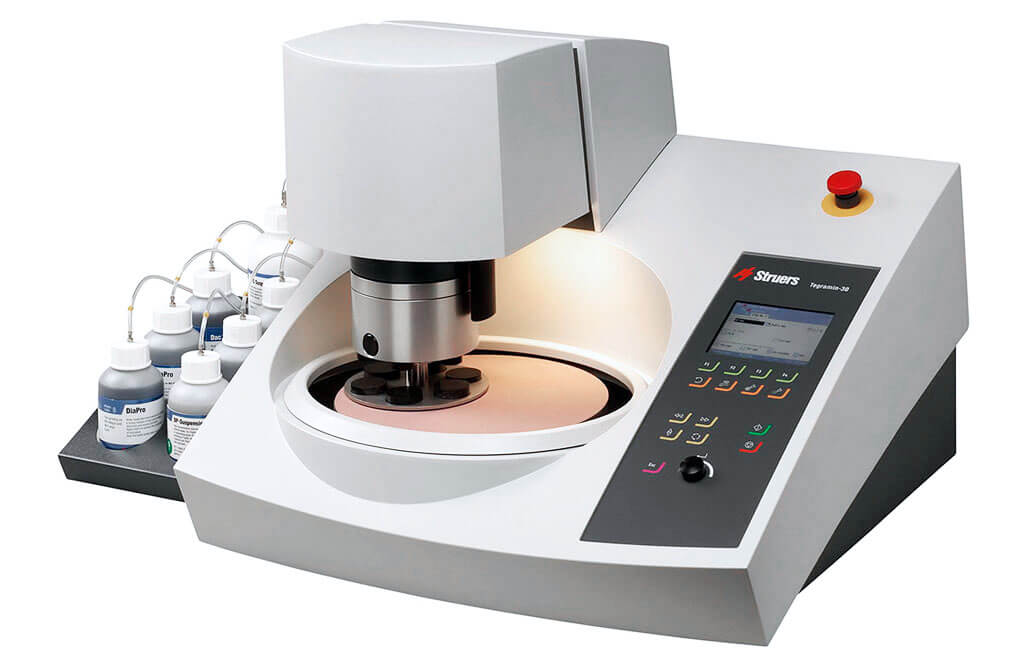
\includegraphics[width=0.5\textwidth]{fig/polishing/Tegramin.jpg}
    \caption{Struers Tegramin polishing machine}
    \label{fig:tegramin}
\end{figure}


\subsection{Stress and cracking}

Cracks forming in the core and cladding material was a problem encountered during polishing of the fibers. It is well documented that the as-drawn fibers contain stress, but it remains an open question in the group whether the cracking observed during polishing results solely from internal stress, or may also be caused by forces experienced during the polishing procedure \cite{Healy2018AFibres, Fokine2017LaserFibers, LapointeElectricalFibres, KristinKristin_thesis_final}. 
%Sources of Stress:
Stress is always formed in MCD fibers due to the different coefficients of thermal expansion of the core and cladding. There are further dynamics during the drawing process, including the interplay between the softening glass cladding and the expansion of the core as it solidifies that will effect the residual stresses in the fiber \cite{Healy2018AFibres}. This can lead to both tensile and compressive strain. Further annealing, after the draw, that reduces grain boundaries or transforms silicon from the amorphous to crystalline state will reduce the volume of the core and modify the stress \cite{Zhao2017EffectFibre}. This illustrates a method of controlling the stress in the fiber, and laser annealing has been used to create bandgap modification in Si \cite{Healy2014ExtremeFibres} and to directly write bragg gratings into the fiber core \cite{Fokine2017LaserFibers}. This problem has been partially addressed with the use of interface modifiers which prevent a strong bond from forming between the Si core and Si02 cladding \cite{Gibson2013AlkalineFibers}, however this has not been able to entirely eliminate the stress.. 
 Work by Zhao has shown that the stresses are concentrated in a ring near the core cladding interface \cite{Zhao2018EffectsFiber}. It was found that furnace annealing led to a reduction in stress, with greater reduction for increasing temperature. However these results should be treated carefully when comparing to our fibers as the as-drawn fibers used in this study were shown to have a low degree of crystallinity, and no interface modifier was used. The improvements in crystalinity of the core shown after the annealing process could be a factor leading to the reduction in stresses that may not be found in highly crystaline samples. However, heating the glass above the glass transition temperature and allowing for a slower cooling time then experienced in the fiber draw should have some impact on the stresses.

\begin{figure}[h]
    \centering
    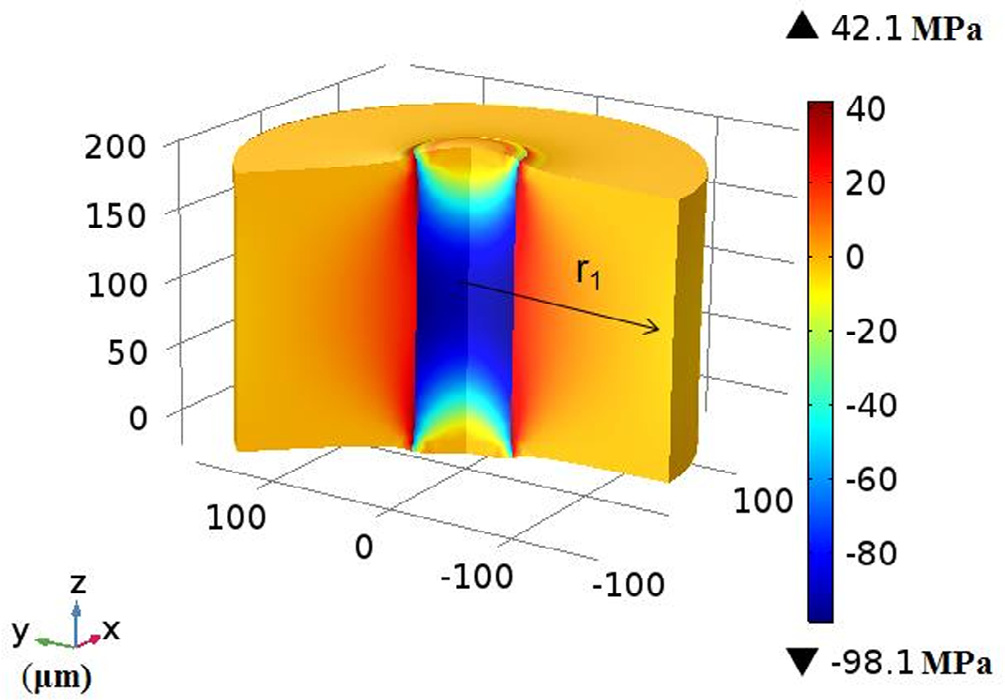
\includegraphics[width=0.5\textwidth]{fig/polishing/stress_simulation.png}
    \caption{Simulated results of stress in a Silica clad Germanium core fibre with no interface modifier, showing how stress may be distributed in a fiber. The core is $70\si{\micro\meter}$ and cladding $310\si{\micro\meter}$. Reprinted from \cite{Zhao2017EffectFiber}}
    \label{fig:my_label}
\end{figure}

To investigate the impact of furnace annealing on our samples, silicon core fibers were chosen to represent a range of core diameters and core cladding ratios. These fibers were heated in a muffle furnace to 1200 with a rate of ?, held for ? minutes and cooled with a  rate of ?. These fibers were then machine polished using diamond abrasive under the same conditions as the untreated fibers. 

To test if the polishing procedure was causing cracking, thin Si wafers (specifics) were mounted in epoxy and machine polished with the same parameters as used on the fibers. Experimentally it was not possible to polish a wafer down to fiber dimensions, but the use of large wafers would expose any significant forces involved if they were to crack during polishing.

%results: 


%Annealing, Recrystalization, core-cladding ratio. %discussion on stress observations why less in redrawn fibers, annealed fibers?

\section{Lithography on Fibers}
\subsection{Maskless Lithography}
Maskless Lithography, or direct laser writing (DLW) is an emerging form of lithography that allows for patterns to be directly written from a digital image to the resist layer without the use of a conventional photomask. Both electron beams and laser light are options for exposing the resist. Electron Beam Lithography (EBL) is a staple of nanofabrication and is capable of writing nanoscale size features. The downside is long write times (typically several hours for a $6$ inch wafer), and the sensitivity to several beam parameters that effect the exposure. Alternatively a laser and a digital micromirror device DMD can be used to pattern features down to $500 \si{\micro\meter}$. The DMD greatly increases the write speed as compared to an EBL as the mirror projects and exposes a small area of the pattern at a time instead of writing point by point. Additional benefits of direct laser writing is the compatibility with conventional resists used for UV lithography, and the ability to operate without a vacuum. For this study an MLA150 maskless alligner from Heidelberg instruments with $\SI{375}{\nm}$ and $\SI{405}{\nm}$lasers is primarily used. Alternatively a Heidelberg MLA100 with $\SI{10}{\watt}$ $\SI{365}{\nm}$ UV LED. A resolution test, shows the ability to achieve $ 1 \si{\micro \meter}$ features in man-440 resist \ref{fig:resolution_test}. 

\begin{figure}[!htb]
    \centering
    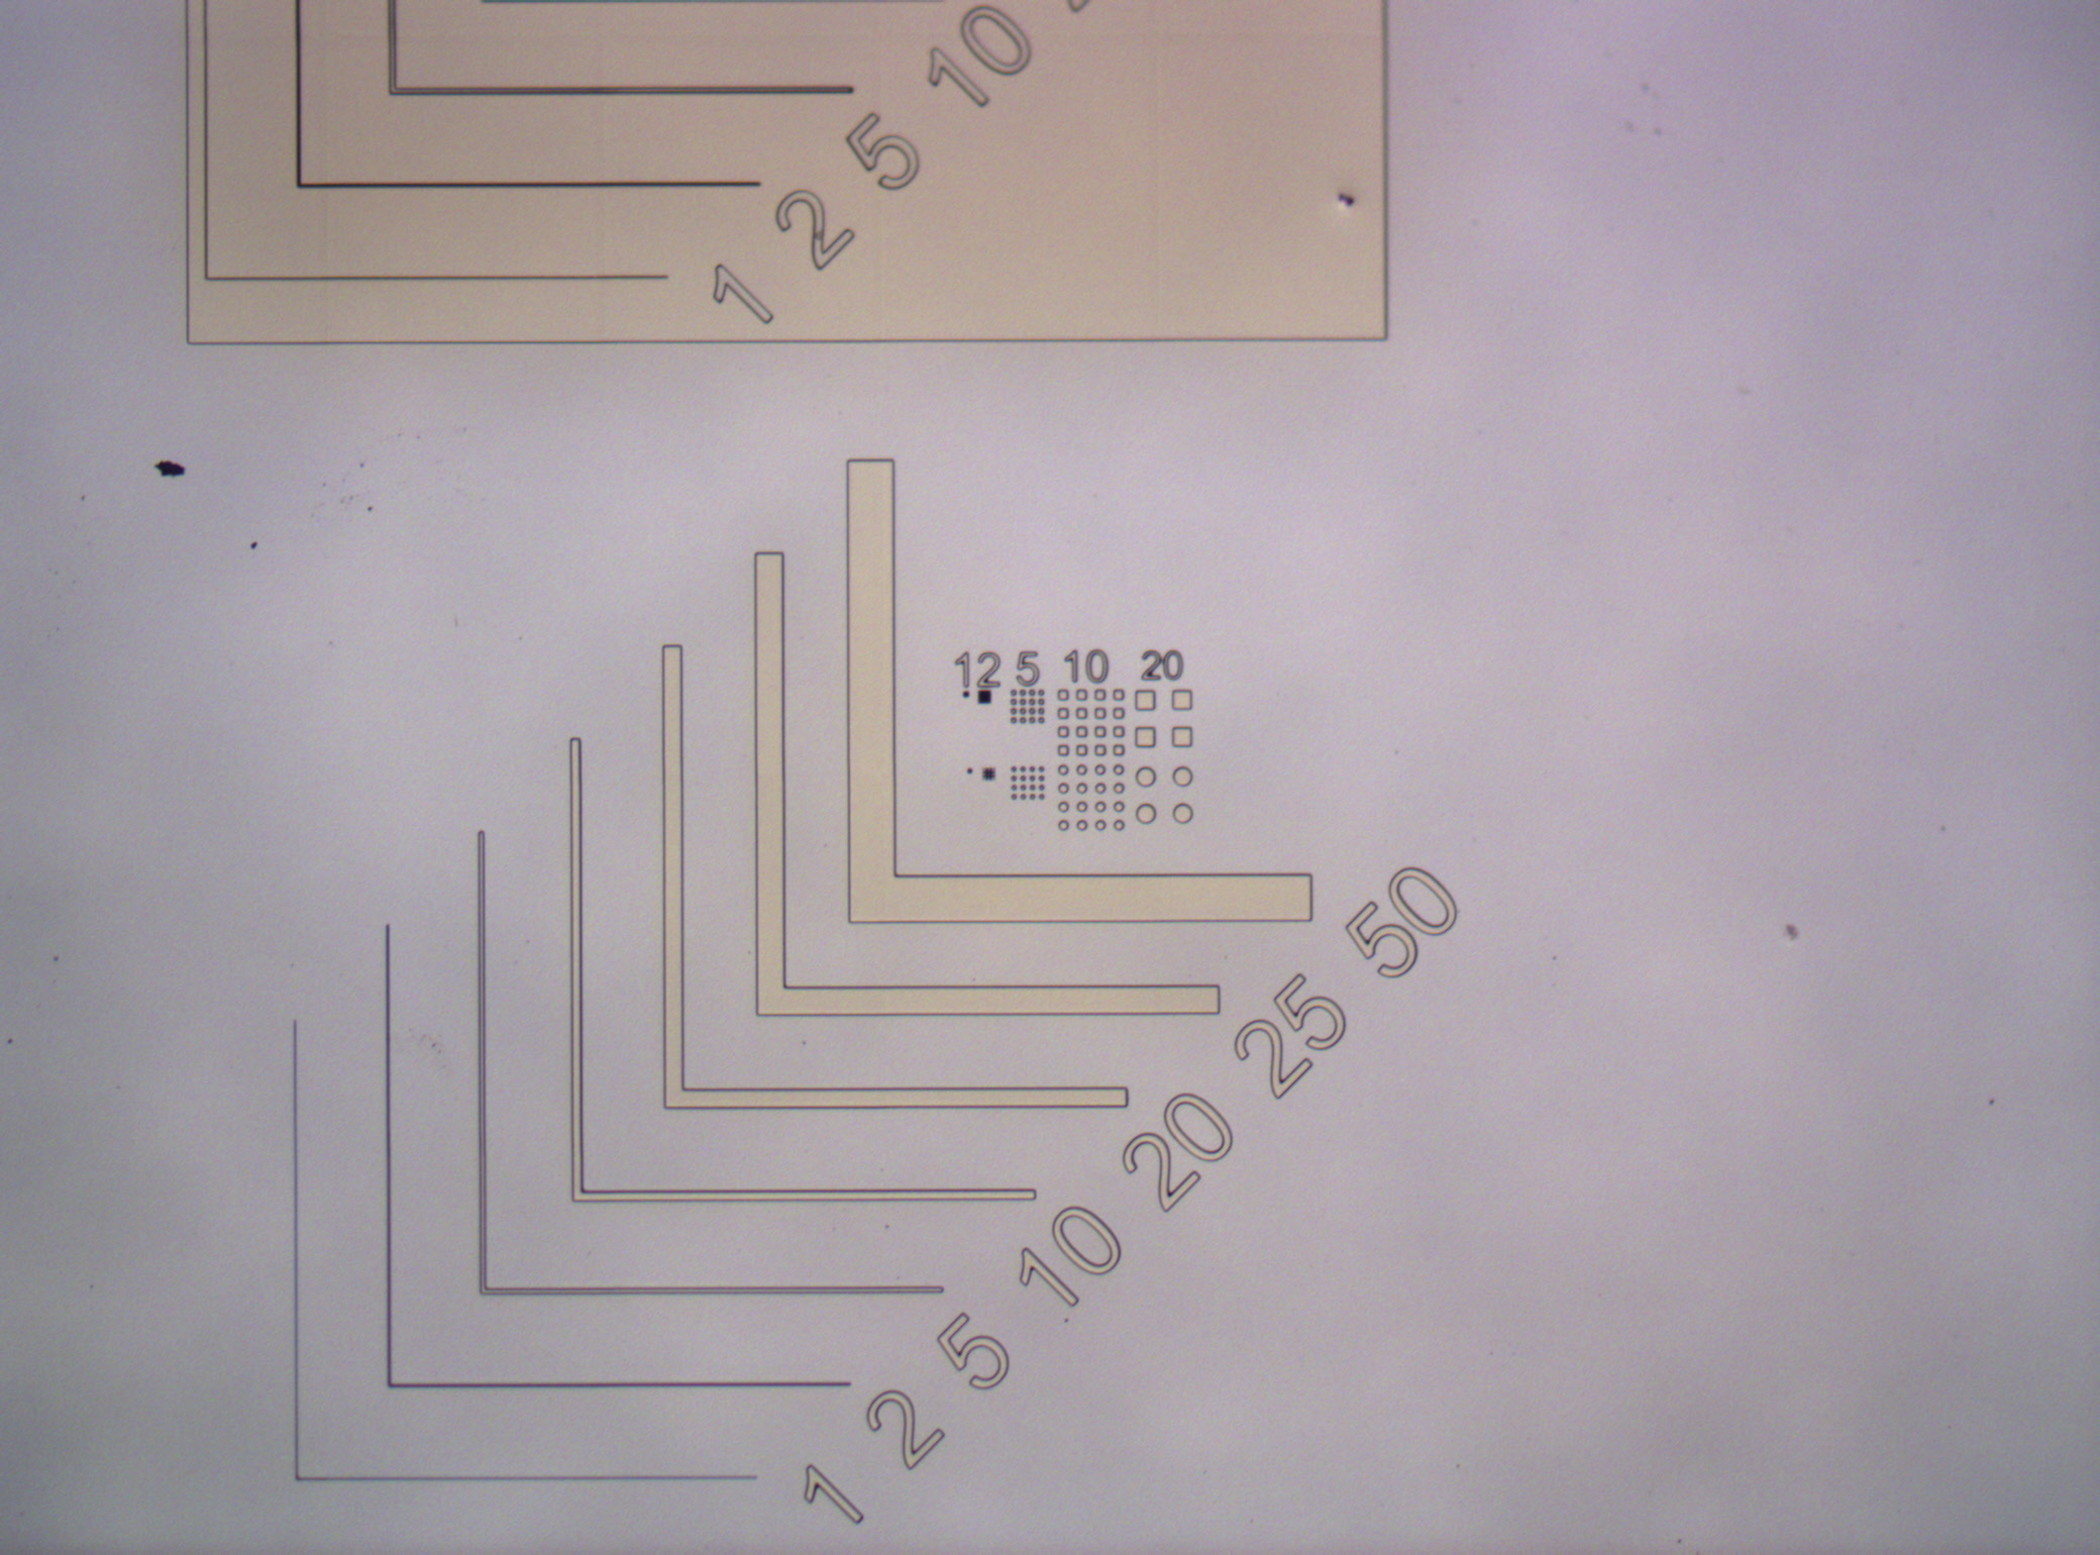
\includegraphics[width=\textwidth]{fig/Results/resolution_test.jpg}
    \caption{Resolution test with Man-440 photo resist on a Si wafer exposed at  $\SI{3200}{\milli \joule \cm^{-2}}$ at $\SI{365}{\nm}$. The numbers indicate the width of the line in microns, and the top of the image shows negative structures, while the bottom shows positive lines on the grey Si background.}
    \label{fig:resolution_test}
\end{figure}

Direct laser writing has several major advantages over conventional lithography for patterning on fibers. The use of a digital pattern allows for customization for each individual fiber. As the fiber diameter and available lengths of continuous core varied, it was necessary to adjust the pattern to obtain an optimal contact spacing, and space the contacts in available areas between cracks in the core. The MLA150 and MLA100 allow for the pattern to be alligned with the substrate with $\SI{500}{\nm}$ accuracy. This allows for precise positioning of the pattern with the fiber cores. 

\subsection{Lithography on Epoxy}
It was necessary to develop a procedure for the deposition of contacts on fibers. While conventional lithogrpahy is primarily used for planar Si wafers, our samples varied in height, and were between 2-5 mm in thickness. Due to the relief of the samples it was necessary to choose a resist that could create a continuous layer over variations in height in the sample. As the fiber in polished samples was up to several microns in height, Man-440 negative tone photoresist was choosen. This resist is designed for a thickness of $\SI{4.1}{\micro \meter}$ and because it is a negative resist it provides for easy lift off. Lift-off is performed in acetone, and as the epoxy shows some instability it acetone a quick liftoff time is desired. The Man-440 resist showed good adhesion to epoxy substrate but small unsupported features such as thin lines on Si and glass occasionally delaminated from the surface. A test was performed of other available resists in this thickness range but none showed suitable liftoff times. [Table of resists here] 
\subsubsection{Prebake and exposure}
See the appendix for more details on lithography procedures.

A prebake time and temperature is given of $\SI{95}{\celsius}$ and $\SI{300}{\second}$ for a contact hotplate and $\SI{100}{\celsius}$ for  $\SI{30}{\minute}$ in an oven. 
 Due to the thickness of the substrate and lower thermal conductivity as compared to a Si wafer an oven bake at the suggested values was used. However these results led to substantially longer development times. As the exposed resist is also removed at a finite rate during development, in a process called dark erosion, extensive development time leads to a thinner resist layer. It was found that a prebake on a contact hotplate gave good results, indicating that the prebake was not extremely sensitive to the sample thickness and thermal conductivity. 
 
 The resist was developed using micro-chemicals 
 There was some difficulty in finding the correct development time. Initially development times were substantially longer than the manufactures value and were not leaving a completely clean surface when removed. The available developer was expired by two years, and it was found that the development times changed substantially when a new bottle with the same expiration date was used. After several weeks, participate would form in the bottle and the development time would again increase. The developer contains a surfactant to help with the removal of exposed resist. It appears that the resist left more residues as the resist aged, possibly indicating a reduction in surfactants as the developer aged. To counter these issues, and promote proper adhesion of the deposited contacts, a plasma clean was used after development to ensure a clean surface. Plasma cleaning can also remove the cross linked resist thus the resist height was checked with a stylus profilometer before and after cleaning. No noticable removal was found for the cleaning times used. 
 \FloatBarrier
\section{Permanent Resist Underlayer}
A remaining problem with the sample preparation is cracking in the glass cladding that impedes the path of the electrical contacts. This consistently happens in the form of a parallel crack propagating on at least one side of the core. Cracking becomes more severe in samples with a larger core to cladding ratio, and in hand drawn samples. Not only does this limit the contact spacing and the number of measurements that can be made on one sample, it also affects the ability to make hall measurements, as the hall pattern requires contacts on either side of the fiber. It is sometimes the case that only a small amount of a particular sample is drawn, and then each sample becomes more important, and a failure during preparation will set back the work significantly. Further if we desire to create structures or junctions within the fiber and characterize the core at the exact point the chances of cracking preventing measurement of the fiber are substantially higher. Due to the small size of the cracks, it is unlikely that filling them with a method such as vacuum impregnation with epoxy would be successful. Further this would require a second polishing step to remove this new layer from the core for electrical measurements.

 
 
\begin{wrapfigure}{r}{0.5\textwidth}
 %h here H requires float, exactly here, h! overide latex
\centering
\begin{subfigure}{.5\textwidth}
  \centering
  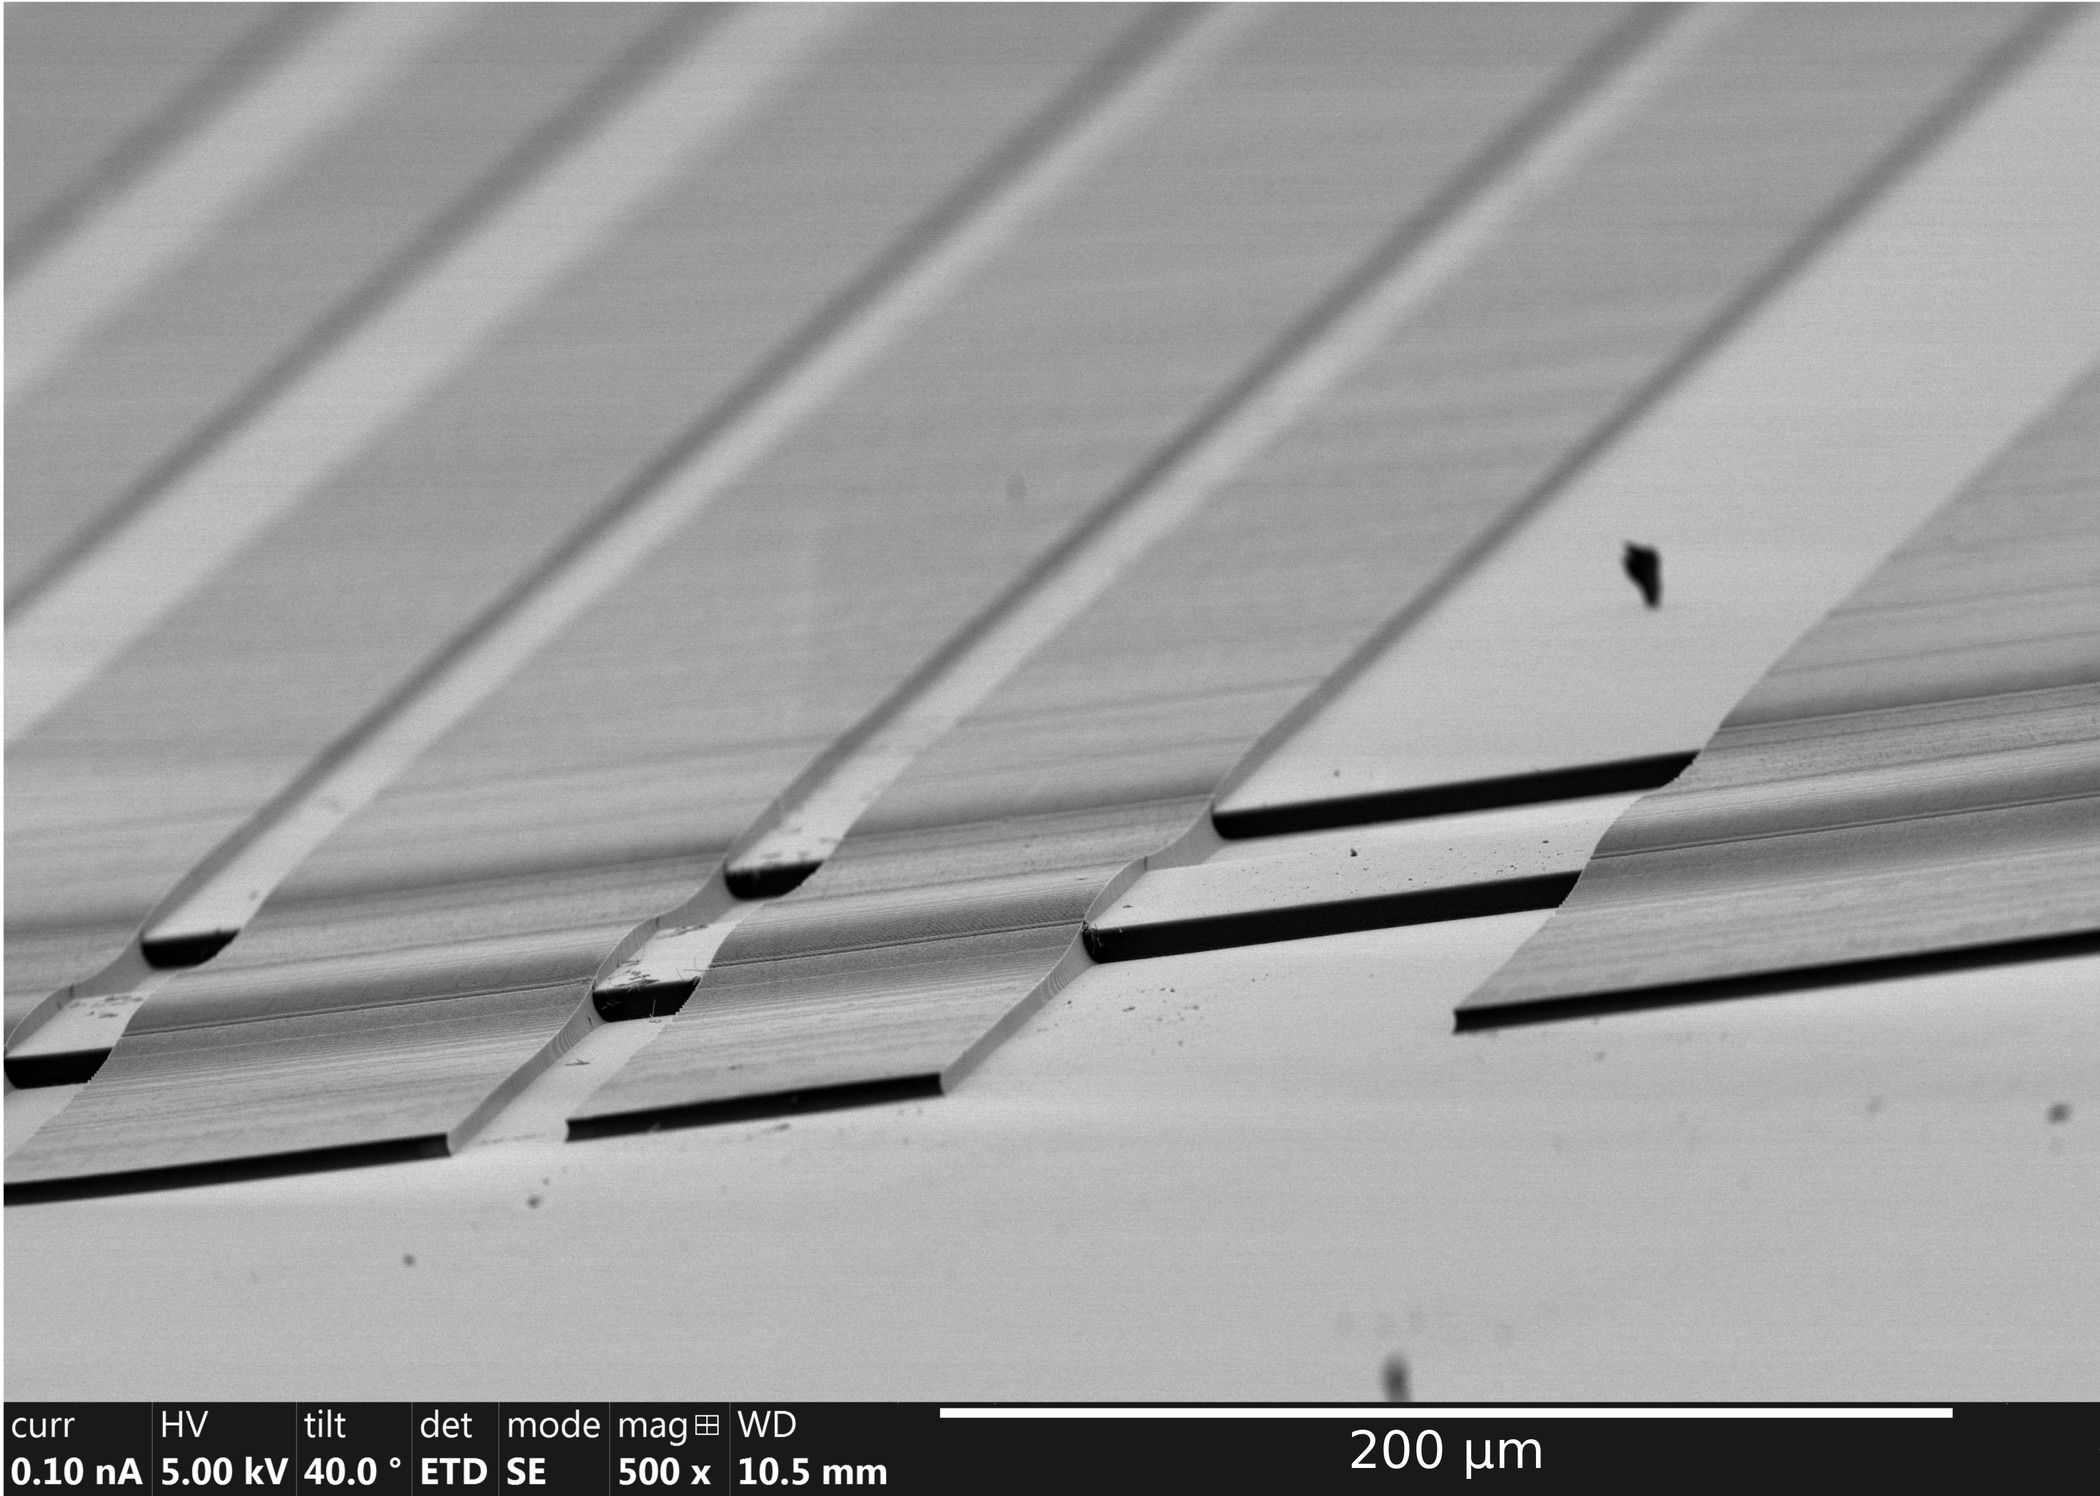
\includegraphics[width=\linewidth]{fig/mr-DWL/sem_mr-dwl-2.jpg}
  %\caption{1a}
  \label{fig:sfig1}
\end{subfigure}% %blank line makes figures vertical

\begin{subfigure}{.5\textwidth}
  \centering
  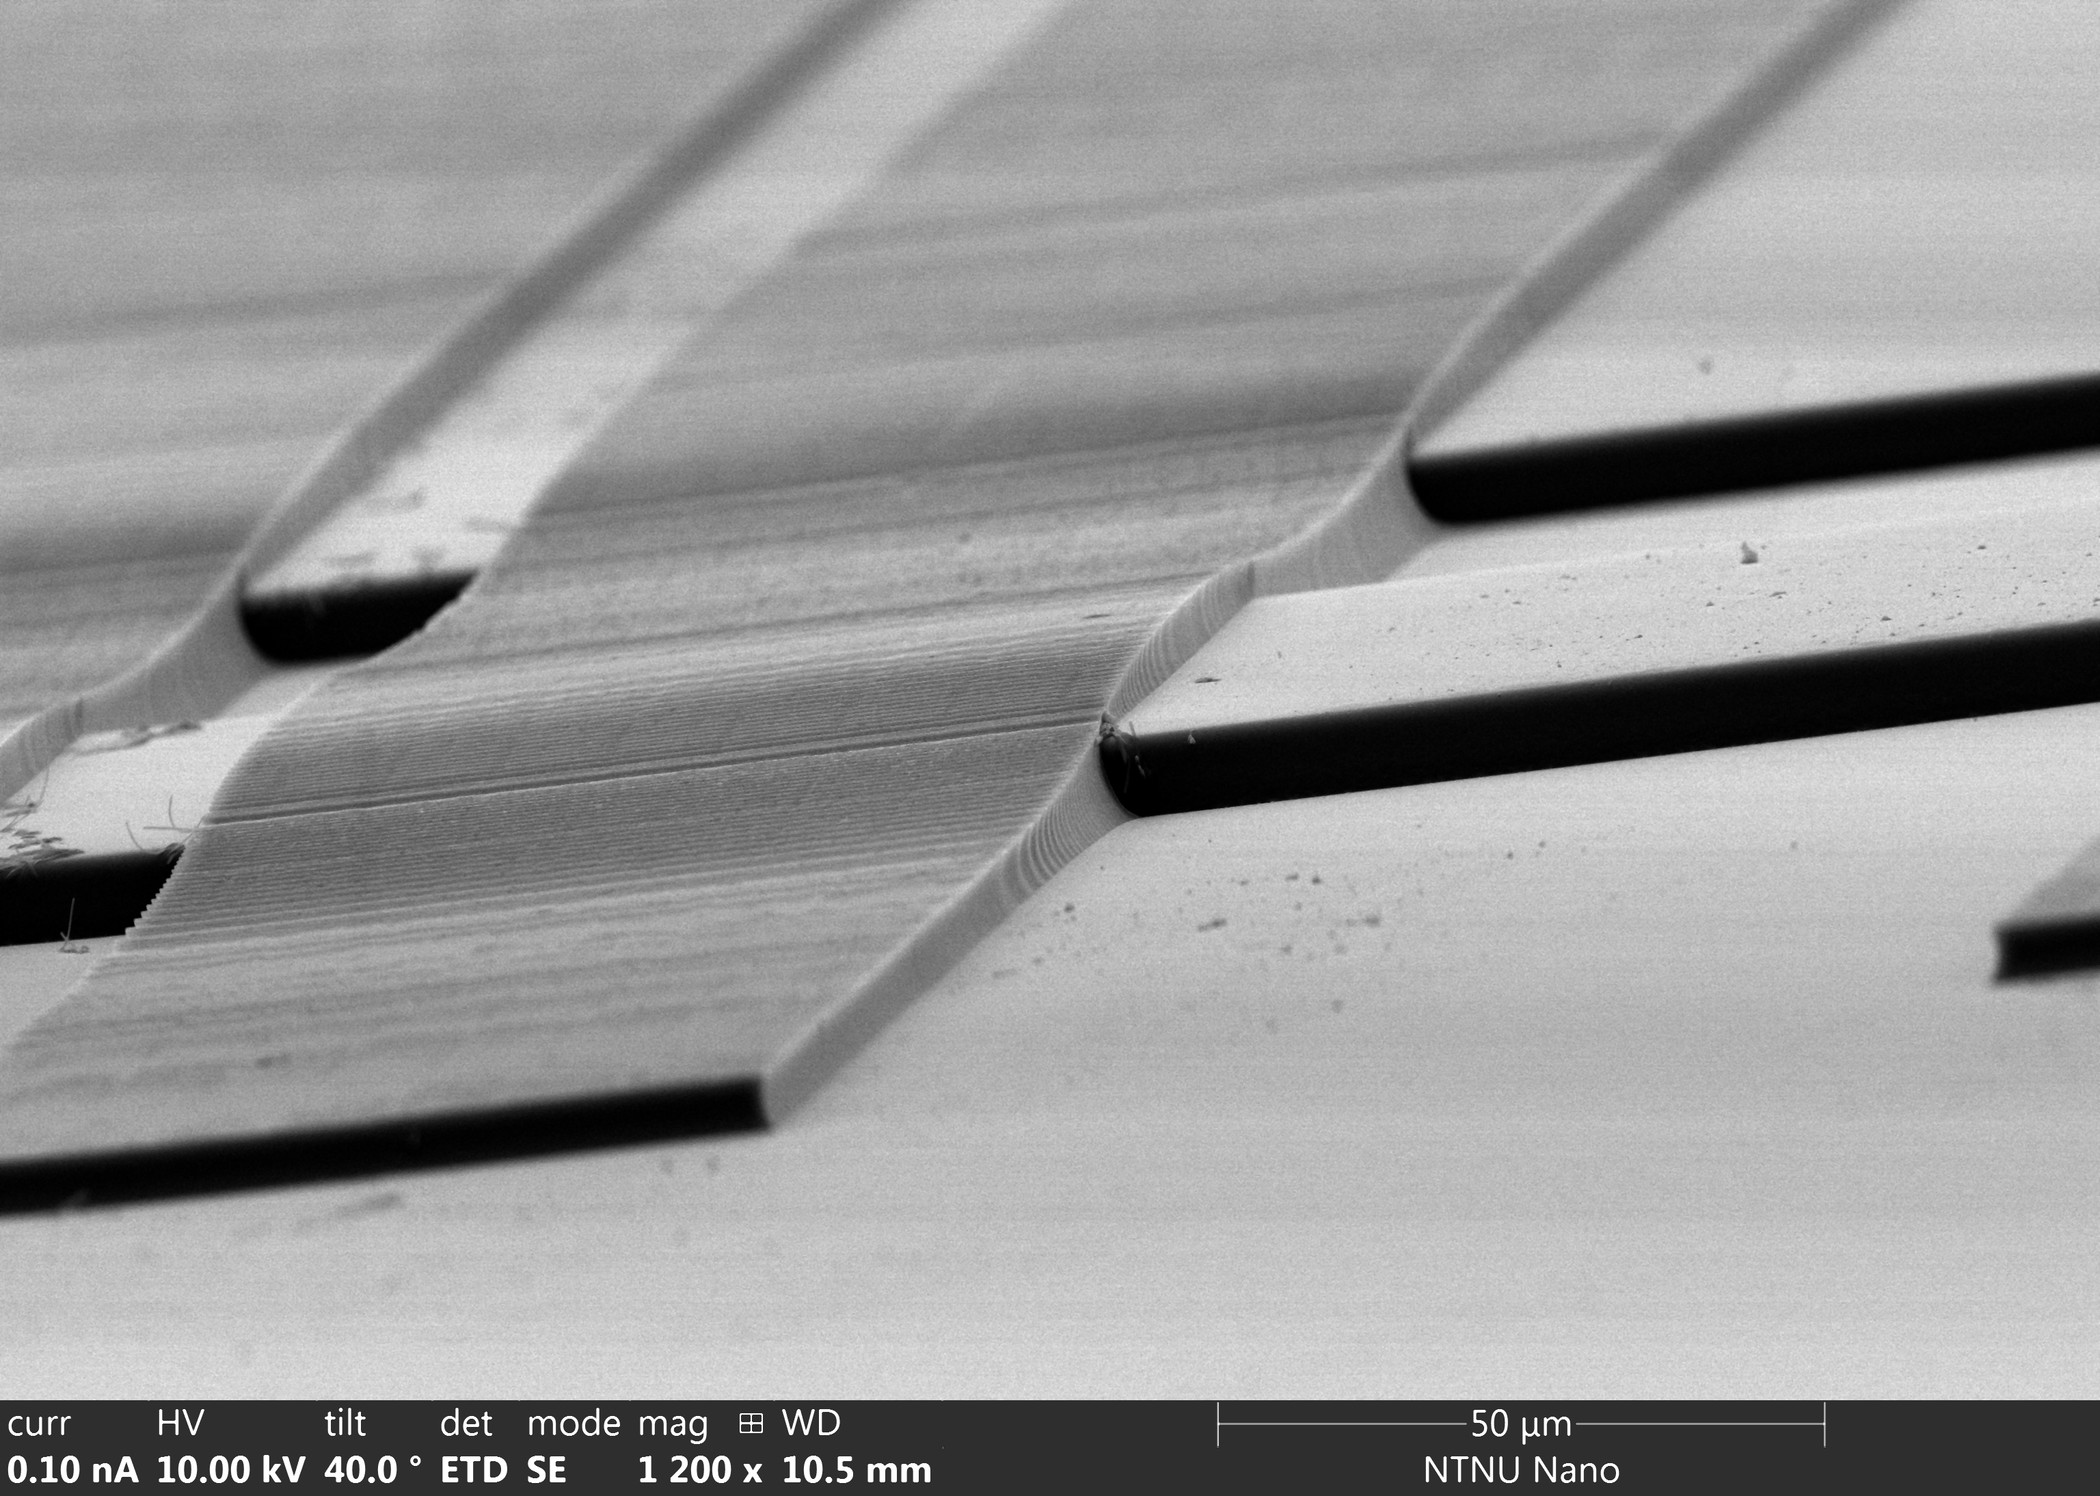
\includegraphics[width=\linewidth]{fig/mr-DWL/sem_mr-dwl.jpg}
  %\caption{1b}
  \label{fig:sfig2}
\end{subfigure}
\caption{$5um$ mr-DWL resist structures coated with a $4um$ man440 layer, demonstrating the possibility of patterning resist structures over a high step edge. }
\label{fig:fig}
\end{wrapfigure}

While photoresist is mainly used for masking purposes, adding a permanent layer of resist would create a smooth surface and without coating the core, and has the advantage of integrating easily with the current process. A second lithography step would add little to the preparation time. The challenges are that the resist layer must be stable in solvent during a second liftoff process and that the contacts deposited over the resist, adhere well and can create continuous coverage of the resist step edge. For the latter a positive resist would be the ideal choice due to the positive sidewall profile. Further a grayscale resist such ma-p1275g  would allow thick films (~100 um) and a controllable positive sidewall profile. While ma-p 1275G would be an ideal choice, tests showed that it was not significantly cross linked after hard baking to withstand an acetone bath. 


The negative photo resists SU-8 and mr-DWL are epoxy based and designed for creating high aspect ratio structures with nearly vertical sidewalls. Further a hardbake step up to  $140 \si{\celsius}$  creates a very stable resist. While the sidewall profile is still negative, tilting the sample during depostion, or using sputtering may allow sufficient step coverage to create a continuous contact. 

\section{Experimental Procedures}
A test sample using mr-DWL 5 was patterned on a Si wafer using the following parameters: spin 3000 rpm patterning $\SI{500}{\milli \joule \cm^{-2}}$ at $405 \si{\micro\meter}$ in the MLA, followed by a hard bake of 30 min $140 \si{\celsius}$. This structure was then coated with $\SI{4}{\micro \meter \cm^{-2}}$ man-440 using the standard recipe described above. 

The procedure was tested on a fiber to examine how the process would work under practical conditions, as the resist thickness, bake temperature and reflections during exposure would all be slightly effected. Electrical contacts were deposited using the standard recipe followed by a sputtered layer of $100 \si{\nano \meter}$. After electrical testing, a further layer of Au was deposited by sputter coating in a small cressington 208 HR B sputter coater, as this was the only method of deposition that allowed for tilting of the sample. Both test samples were analysed by 3d-optical profilometry and SEM. 

\section{MiBots}
An alternative to the Lithographic techniques described, is direct probing of the sample using micro manipulators. Imina Techinology Mibots are vacuum compatible micro manipulators with interchangeable tungsten probes capable of electrical probing. The probe positioning precision is in the nm range and is more than sufficient for fiber measurements. The MiBots have a stage that can be used with an optical or electron microscope. Use with an electron microscope allows for high accuracy in the measurement of the probe spacing. Direct probing has the advantage of eliminating the challenges associated with lithography, including the need to bridge an cracking in the glass fiber and any relief profile and possible chipping at the glass epoxy interface. Problems with metal adhesion to the three different materials (glass,epoxy,core) are substrate is also eliminated. While work has been done to use micromanipulators to characterize semiconductor fibers \cite{Engel2016DirectPhotosynthesis} past experience in our group has found that reliable electrical contact is difficult to achieve. %Ohmic contacts of the manipulators requires sufficient force (look up here). 
Depositing micro contacts along the core should provide a reliable method of contacting the sample while still avoiding many of the problems encountered with larger contacts.  



\begin{figure}[t]
  \centering
    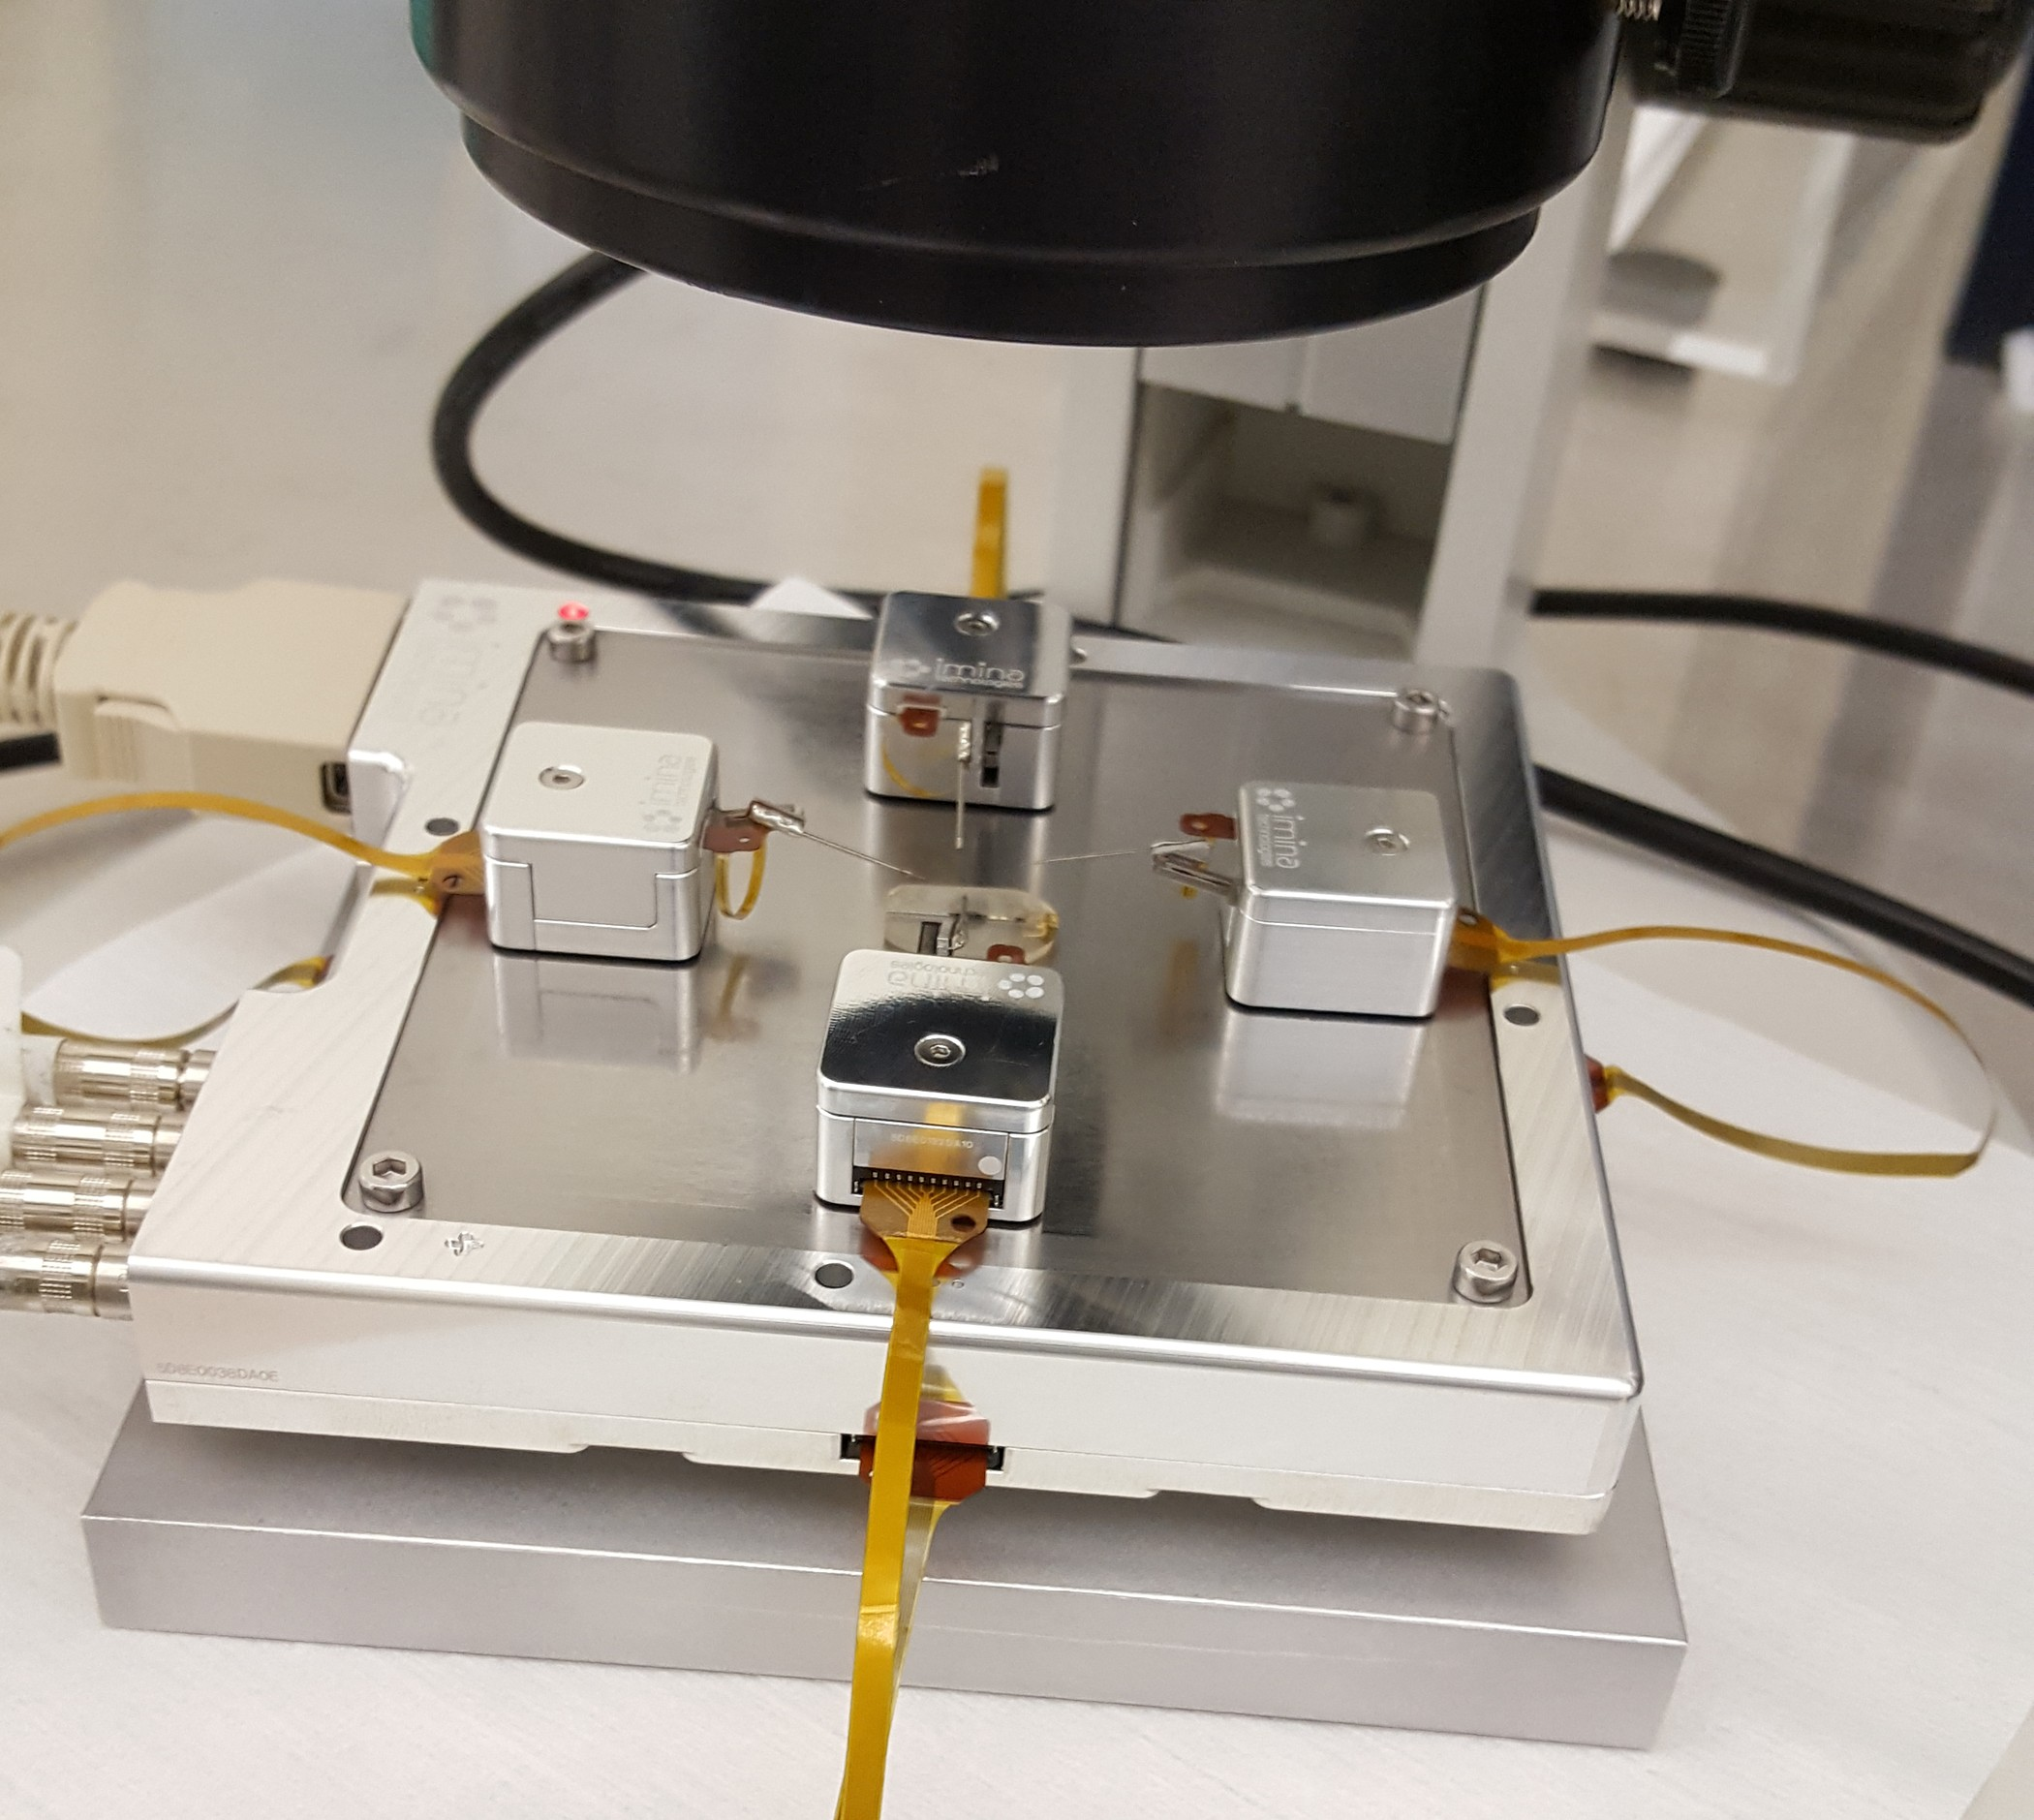
\includegraphics[width=0.7\textwidth]{fig/MiBots/setup.jpg}
 \caption{Mibot stage under an optical microscope.}
\label{mibot}
\end{figure}

\begin{figure}[t]
  \centering
    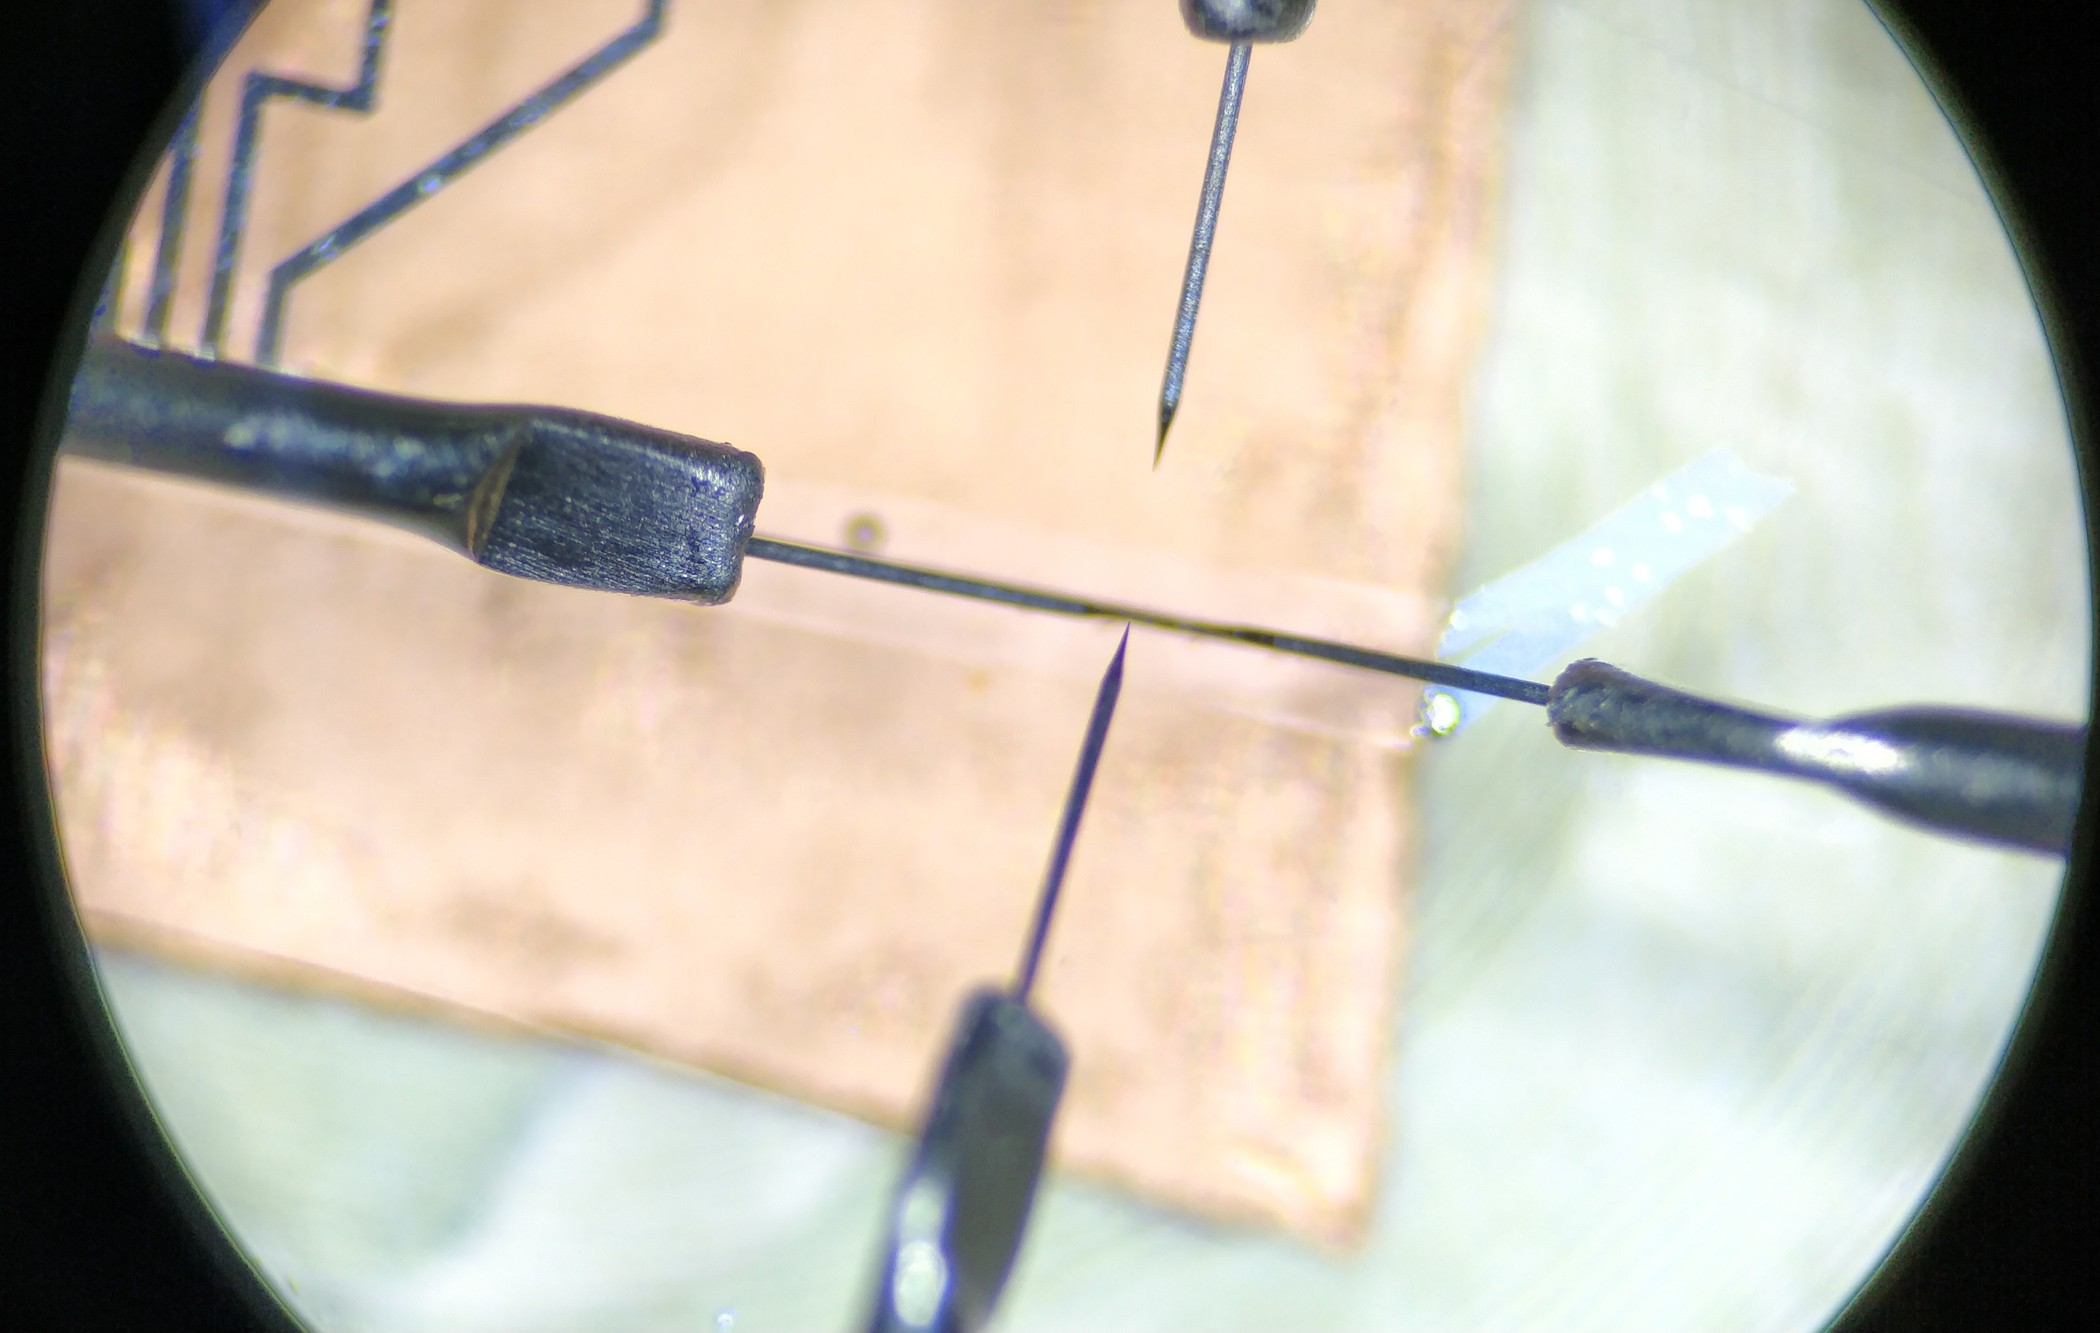
\includegraphics[width=0.7\textwidth]{fig/MiBots/IMG_20190409_143016.jpg}
 \caption{ Operators view through the microscope eyepiece of Mibot with 1 um Probe tips directly contacting the exposed sample core. The two outer current carrying probes are in contact while the voltage probes are raised above the sample.}
\label{mibot}
\end{figure}

\begin{figure}[t]
  \centering
    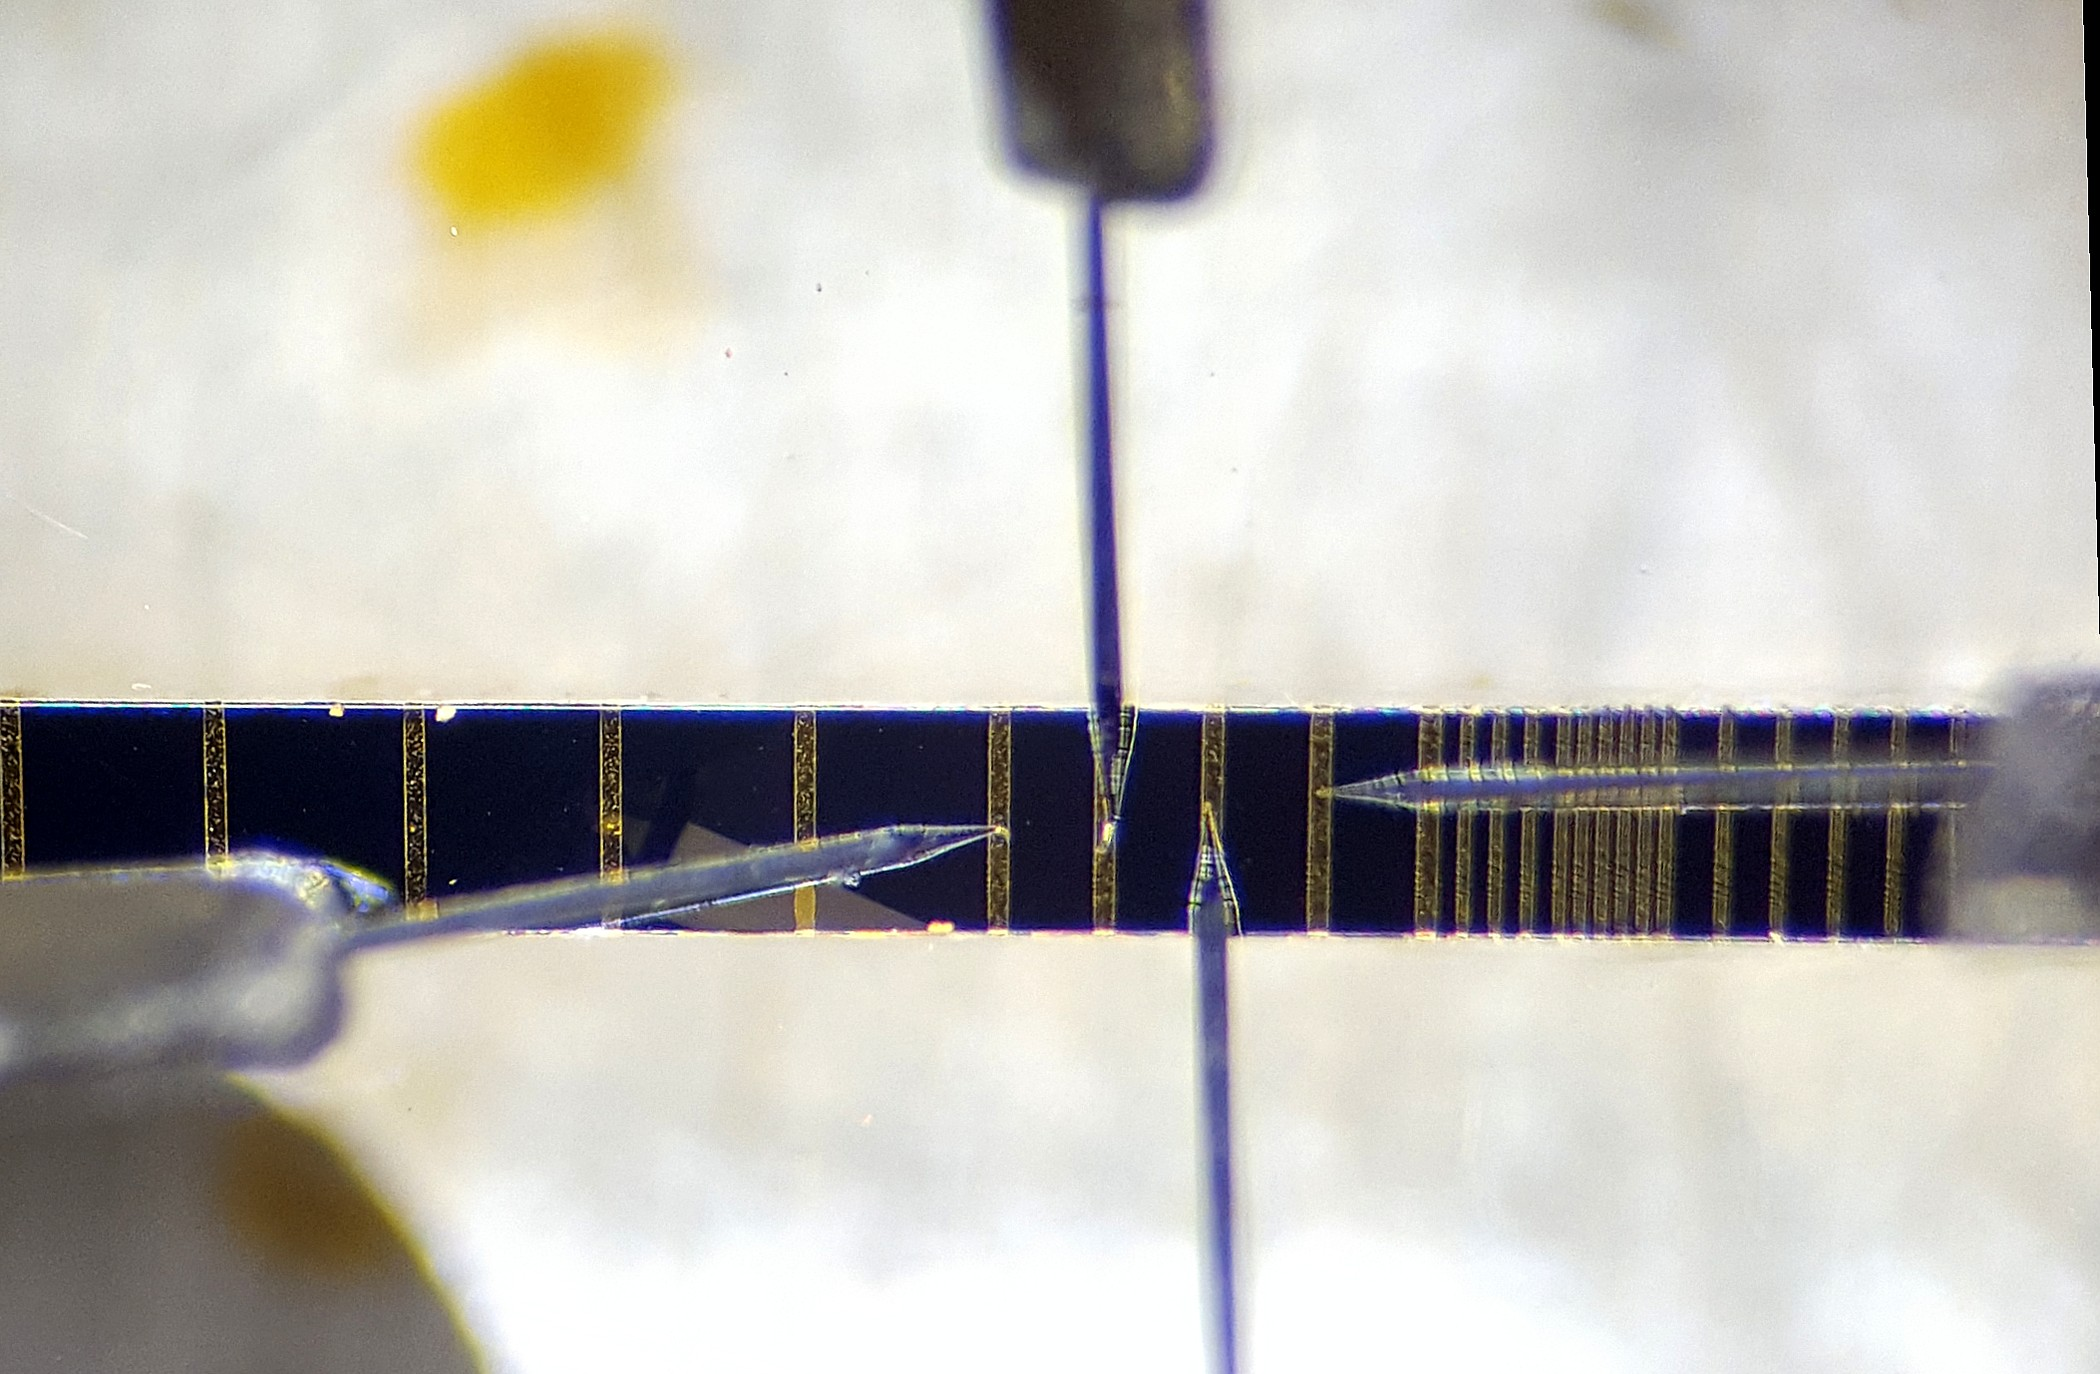
\includegraphics[width=0.7\textwidth]{fig/MiBots/closeup.jpg}
 \caption{Alternative Image for fig 3.6. Test sample with contacts. }
\label{mibot}
\end{figure}

 \cleardoublepage